\documentclass{standalone}
\usepackage{tikz}
\usepackage{ctex,siunitx}
\setCJKmainfont{Noto Serif CJK SC}
\usepackage{tkz-euclide}
\usepackage{amsmath}
\usetikzlibrary{patterns, calc,3d}
\usetikzlibrary {decorations.pathmorphing,decorations.pathreplacing,decorations.shapes}
\begin{document}
\small
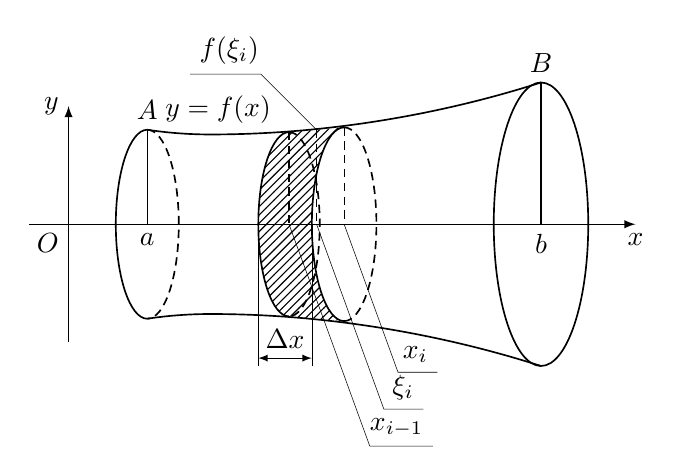
\begin{tikzpicture}[>=latex,scale=1.0]
  \draw[->](-0.5,0)--(7.2,0)node[below]{$x$};
  \draw[->](0,-1.5)--(0,1.5)node[left]{$y$};
  \node at (0,0)[below left]{$O$};
  \draw[semithick](6,0)ellipse(0.6 and 1.8);
  \draw[semithick](1,1.2)arc(90:270:0.4 and 1.2);
  \draw[semithick,densely dashed](1,1.2)arc(90:-90:0.4 and 1.2);
  \draw[semithick](1,1.2)parabola bend(1.8,1.14)(6,1.8);
  \draw[semithick](1,-1.2)parabola bend(1.8,-1.14)(6,-1.8);
  \draw(1,1.2)node[above]{$A$}--(1,0)node[below]{$a$};
  \draw(6,1.8)node[above]{$B$}--(6,0)node[below]{$b$};
  \draw[semithick](2.8,1.17)arc(90:270:0.39 and 1.17);
  \draw[semithick,densely dashed](2.8,1.17)arc(90:-90:0.39 and 1.17);
  \draw[semithick](3.5,1.23)arc(90:270:0.41 and 1.23);
  \draw[semithick,densely dashed](3.5,1.23)arc(90:-90:0.41 and 1.23);
  \draw[densely dashed](2.8,1.17)--(2.8,0)(3.5,1.23)--(3.5,0)(3.15,1.2)--(3.15,0);
  \fill[pattern=north east lines](2.8,1.17)arc(90:270:0.39 and 1.17)--(3.5,-1.23)arc(270:90:0.41 and 1.23)--cycle;
  \draw[very thin](2.41,0)--(2.41,-1.8)(3.09,0)--(3.09,-1.8);
  \draw[very thin,<->](2.41,-1.7)--(3.09,-1.7)node[midway,above]{$\Delta x$};
  \draw[very thin](2.8,0)--++(-70:3.0)--++(0.8,0)node[above left]{$x_{i-1}$};
  \draw[very thin](3.15,0)--++(-70:2.5)--++(0.5,0)node[above left]{$\xi_i$};
  \draw[very thin](3.5,0)--++(-70:2.0)--++(0.5,0)node[above left]{$x_i$};
  \draw[very thin](3.15,1.2)--++(135:1.0)--++(-0.9,0)node[above right]{$f(\xi_i)$};
  \node at (1.9,1.15)[above]{$y=f(x)$};
\end{tikzpicture}
\end{document}